\title{Mandelbrot Set}
\date{}

\documentclass[12pt]{article}

\usepackage[italian]{babel}
\usepackage[T1]{fontenc}
\usepackage[utf8]{inputenc}
\usepackage{graphicx}

\usepackage{amsmath,systeme}

\begin{document}
\maketitle

\newpage

\section{Introduzione}

Il progetto riguarda l'elaborazione del frattale \emph{Mandelbrot set} attraverso tre diversi livelli di parallelizzazione del calcolo:
\begin{itemize}
\item Nessuna parallelizzazione 
\item Parallelizzazione CPU
\item Parallelizzazione GPU
\end{itemize}
L'insieme di \emph{Mandelbrot} è l'insieme dei numeri complessi $c$ per cui la successione:
$$
\begin{cases}
	z_0 = 0\\
	z_{n+1} = z_n^{2} + c
\end{cases}
$$
è limitata.

\begin{figure}[h]

\includegraphics[width=\textwidth]{mandelbrot.jpg}
\centering
\end{figure}

\section{Parallelizzazione}

Parallelizzare la computazione è relativamente facile in quanto la stima della convergenza di un singolo punto è indipendente dalla stima della convergenza degli altri, per cui non c'è bisogno di sincronizzazione e comunicazione tra thread.

La versione che sfrutta la parallelizzazione \emph{CPU} si limita a suddividere l'immagine in $N$ righe e a computarle mediante $N$ thread.

La parallelizzazione GPU è, invece, stata implementata sfruttando \emph{CUDA}, da cui si è realizzato un insieme di blocchi della stessa dimensione dell'immagine da renderizzare, con un thread ciascuno.

\section{Benchmark}

Il \emph{benchmark} è stato eseguito modificando la larghezza dell'immagine da renderizzare, mantenendo le proporzioni, in modo da aumentare il numero di operazioni in modo asintotico al quadrato della larghezza, nel caso single thread.

Si nota che la GPU si rivela essere, sempre, il dispositivo migliore per affrontare questo tipo di computazione.

\begin{figure}[h]
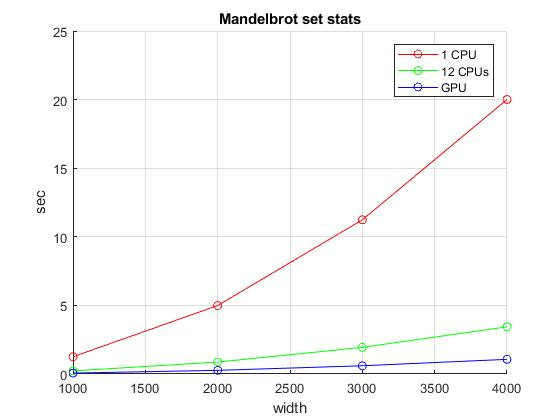
\includegraphics[width=\textwidth]{MandelbrotStats.jpg}
\centering
\end{figure}

\section{Conclusioni}
Si è potuto osservare come la GPU permetta di parallelizzare i calcoli molto più della CPU e che per questo tipo di computazione è la scelta migliore. Con una buona GPU sarebbe possibile sviluppare anche un ingrandimento, animato, real time del frattale

\end{document}
